\setcounter{chapter}{-1} % Para empezar a contar en 0

\chapter{Introducción}

La mayoría de ecuaciones diferenciales han sido planteadas por campos como la física. Veamos el caso de un péndulo:

\begin{figure}[H]
    \centering
    \begin{subfigure}{0.3\textwidth}
        \centering        
        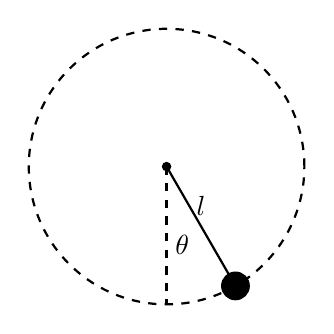
\begin{tikzpicture}
            \centering

            \def\radius{1.75}
            \def\angulo{150}

            % Desactiva los caracteres conflictivos
            \shorthandoff{>} % Para poner puntas de flecha

            \draw[thick, dashed] (0,0) circle (\radius);
            \filldraw (0,0) circle (1.5pt);
            \filldraw ({sin(\angulo)*\radius}, {cos(\angulo)*\radius}) circle (5pt);
            \draw[thick] (0,0) -- ({sin(\angulo)*\radius}, {cos(\angulo)*\radius}) node[midway, above] {$l$};
            \draw[thick, dashed] (0,0) -- (0,-\radius);
            \node at (0.2,-1) {$\theta$};

        \end{tikzpicture}

        \vspace*{0.25cm}
    \end{subfigure}
    \hfill
    \begin{subfigure}{0.6\textwidth}%
        Las condiciones que definen el péndulo son $g >0$, ya que se encuentra en la Tierra, $l$ que es la longitud del péndulo y $\theta$ que es el ángulo con respecto a la vertical.

        La ecuación que define el ángulo a lo largo del tiempo es la siguiente:
        \begin{gather*}
            \theta''(t) + \frac{g}{l} \sen(\theta(t)) = 0
        \end{gather*}
    \end{subfigure}
    \hfill
\end{figure}

Esta es una ecuación diferencial de segundo orden (ya que aparece una segunda derivada). En ella tenemos que $t$ es la variable independiente y $\theta$ es la incógnita o variable dependiente (que es una función).

Si estudiamos las soluciones de esta ecuación tenemos 
\begin{align*}
    \theta(t) &= 0, \ t\in \bb{R} \text{ es una solución (trivialmente)}\\
    \theta(t) & =\pi, \ t \in \bb{R} \text{ es también solución}\\
    \theta(t) & =2n\pi,\ \theta(t) =n\pi, \ t \in \bb{R},\ n \in \bb{Z} \text{ son infinitas soluciones}\\
\end{align*}

De esta forma podemos ver que una ecuación diferencial puede tener infinitas soluciones.

\begin{definicion}
    Podemos definir una \textbf{ecuación diferencial de primer orden} como la relación funcional dada por 
    \begin{gather*}
        \Phi (t, x(t), x'(t)) = 0
    \end{gather*}
    donde $t$ es la \textbf{variable independiente} y $x=x(t)$ es la \textbf{variable independiente} o \textbf{incógnita}.
\end{definicion}

\begin{ejemplo}
    Consideremos la ecuación diferencial dada por
    \begin{gather*}
        x(t) + x'(t)^2 = 1
    \end{gather*}
    Podemos definir\footnote{Notación física} $\Phi = \Phi(t,x,y) = x^2 + y^2 -1$, o equivalentemente\footnote{Notación moderna (matemática)}
    \begin{align*}
        \Phi : D \subset \bb{R}^3 &\rightarrow \bb{R} \\
        (t,x,y) & \mapsto \Phi(t,x,y) = x^2 + y^2 -1
    \end{align*}
    Estudiemos las soluciones a esta ecuación:

    \begin{figure}[H]
        \centering
        
        \begin{subfigure}{0.3\textwidth}
            \centering
            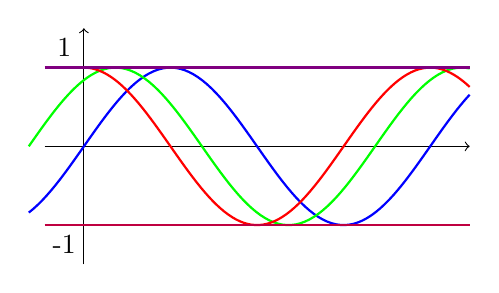
\begin{tikzpicture}
                % Desactiva los caracteres conflictivos
                \shorthandoff{>} % Para poner puntas de flecha

                \def\escalax{0.7}
                % Ejes
                \draw[->] (-0.5,0) -- (\escalax*7,0);
                \draw[->] (0,-1.5) -- (0,1.5);
            
                % Gráfica del seno
                \draw[blue, thick, domain=-1:7, samples=100] plot (\escalax*\x,{sin(\x r)});

                % Gráfica del seno trasladada
                \draw[green, thick, domain=-1:7, samples=100] plot (\escalax*\x,{sin(((\x+1) r))});
            
                % Gráfica del coseno
                \draw[red, thick, domain=0:7, samples=100] plot (\escalax*\x,{cos(\x r)});

                % Horizontales
                \draw[violet, thick] (-0.5,1) --(\escalax*7,1);
                \draw[purple, thick] (-0.5,-1) --(\escalax*7,-1);
            
                    
                % Etiquetas de los valores en el eje y
                \node at (-0.25,1.25) {1};
                \node at (-0.25,-1.25) {-1};
            \end{tikzpicture}

            \vspace*{0.5cm}
    
        \end{subfigure}
        \hfill
        \begin{subfigure}{0.6\textwidth}%
            \begin{itemize}
                \item[\textcolor{blue}{$\bullet$}] $x(t) = \sen(t)$, $t \in \bb{R}$
                \item[\textcolor{red}{$\bullet$}] $x(t)= \cos(t)$, $t \in \bb{R}$
                \item[\textcolor{violet}{$\bullet$}] $x(t)=1$, $t \in \bb{R}$
                \item[\textcolor{purple}{$\bullet$}] $x(t)=-1$, $t \in \bb{R}$
                \item[\textcolor{green}{$\bullet$}] $x(t)=\sen(t+c)$, $t \in \bb{R}$ $\forall c \in \bb{R}$ (familia uniparamétrica).
            \end{itemize}
        \end{subfigure}
        \hfill
    \end{figure}

    Podemos construir otra solución uniendo las ya dadas como por ejemplo
    \begin{gather*}
        x(t)=\left\{
        \begin{array}{ccc}
            \cos(t)& \text{ si }& t \geq 0\\
            1&  \text{ si } & t <0
        \end{array}
        \right.
    \end{gather*}
    Esta función es derivable y por tanto solución a la ecuación.

\end{ejemplo}

Típicamente estudiaremos ecuaciones diferenciales de primer orden en \textbf{forma normal}, es decir, ecuaciones que se pueden escribir como
\begin{gather*}
    x'(t) = f(t, x(t))
\end{gather*}
Esto es una subfamilia de las ecuaciones previamente descritas.

\begin{ejemplo}\ 
    \begin{enumerate}[label=\alph*)]
        \item $x'(t)=7x(t)$
        \begin{align*}
            \Phi(t,x,y)&=y-7x \\
            f(t,x) &= 7x
        \end{align*}
        Algunas de las soluciones son $x(t)=0$ (trivial), $x(t)=e^{7t}$ y $x(t)=c \cdot e^{7t},\ \ c, t\in \bb{R}$

        \item $x`(t)=7t$
        \begin{align*}
            \Phi(t,x,y)&=y-7t \\
            f(t,x) &= 7t
        \end{align*}
        Algunas de las soluciones son de la forma $x(t)=\frac{7t^2}{2} + c$, $c, t \in \bb{R}$ (realmente es una integral).
    \end{enumerate}
\end{ejemplo}

\begin{ejemplo}\
    \begin{enumerate}[label=\alph*)]
        \item $x`(t)=\sen(t)$. Sus soluciones son de la forma $x(t)=\cos(t)+c$, $c,t\in \bb{R}$
        \item $x`(t)=\sen(x(t))$. No es tan simple calcular las soluciones (aunque $x(t)=0$, $t\in \bb{R}$ es solución).
    \end{enumerate}
\end{ejemplo}

\begin{definicion}
    Una función diferencial va a venir dada por un 
    \begin{align*}
        \Phi : D \subset \bb{R}^3 &\to \bb{R}\\
        (t,x,y) &\mapsto \Phi(t,x,y) \text{ (continua)}
    \end{align*}
    donde el conjunto $D$ es un abierto de $\bb{R}^3$ conexo llamado \textbf{dominio}.

    Una \textbf{solución} de una ecuación diferencial, $\Phi(t,x(t),x`(t))=0$ será una función de la forma 
    \begin{align*}
        x: I &\to \bb{R}\\
        t & \mapsto x(t)
    \end{align*}
    donde $I$ es un intervalo abierto y $x$ tiene las siguientes propiedades:
    \begin{enumerate}
        \item[(i)] $x(t)$ es derivable en $I$.
        \item[(ii)] $(t,x(t), x'(t))\in D$\ \ \ $\forall t \in I$
        \item[(iii)] $\Phi(t, x(t), x'(t))=0$\ \ \ $\forall t \in I$
    \end{enumerate}
\end{definicion}

\begin{ejemplo}
    \begin{gather*}
        x(t)=\sqrt{2t - 38}, 
        \hspace{2cm} 
        x'(t)=\frac{1}{x(t)}
    \end{gather*}
    ¿Es $t(x)$ una solución de la ecuación dada?
    \begin{gather*}
        \Phi(t,x,y)=y - \frac{1}{x}
        \hspace{2cm} 
        D=\bb{R}\times ]0,\infty[ \times \bb{R}
        \hspace{2cm} 
        I=]19, \infty[
    \end{gather*}

    Tomamos así $D$ porque hay que quitar la discontinuidad que se produce en el plano $\{(t,x,y)\in \bb{R}^3 : x=0\}$ y además tiene que ser conexo ($\bb{R}^3$ sin un plano no es conexo).

    $I$ es el mayor intervalo abierto de $\bb{R}$ en el que $x(t)$ es derivable.

    Además, se verifica que $(t,x(t),x'(t))\in D$\ \ \ $\forall t \in I$ y 
    \begin{gather*}
        x'(t)=\frac{1}{\sqrt{2t-38}}=\frac{1}{x(t)}
    \end{gather*}
    Por lo que se verifica que es solución

\end{ejemplo}

A partir de ahora la notación que utilizaremos para expresar ecuaciones diferenciales será
\begin{gather*}
    \Phi(t,x,x') = 0 \text{ en lugar de } \Phi(x, x(t), x'(t))
\end{gather*}

\begin{ejemplo}
    \begin{align*}
        x&'=3x \hspace{1cm} (\sii x'(t)=3x(t))\\
        x(t)&=c \cdot e^{3t}
    \end{align*}

    En general, tenemos que
    \begin{align*}
        &x = \lambda x  \ \ \text{ tiene por solución }\ \  x(t)=c \cdot e ^{\lambda t}\\
        &x'=\lambda t\ \  \text{ tiene por solución }\ \  x(t)=\frac{\lambda t^2}{2} +c
    \end{align*}

\end{ejemplo}

\begin{prop}
    Dada $x(t)$ solución de $x'=\lambda x$ definida en un intervalo abierto $I$, existe $c\in \bb{R}$ de forma que $x(t)=c \cdot e^{\lambda t}$,\ \ $\forall t \in I$.

    \begin{proof}
        Sea $x(t)$ una solución. Consideramos la aplicación $e^{-\lambda t} \cdot x(t)$ que es derivable por ser producto de funciones derivables y tenemos
        \begin{gather*}
            \frac{d}{dt}\left( e^{-\lambda t} x(t)\right) = -\lambda e^{-\lambda t} x(t) + e^{-\lambda t}x`(t) \overset{(*)}{=}-\lambda e^{-\lambda t} x(t) + e^{-\lambda t}\cdot \lambda x(t) = 0
        \end{gather*}
        donde en $(*)$ he aplicado que $x'=\lambda x$ por ser solución. Al anularse la derivada de una función de clase $C^1(I)$, necesariamente tenemos que $\exists c \in \bb{R}$ tal que $e^{-\lambda t}x(t)=c$\ \ $\forall t \in I$.

        Con esta expresión, dado que la exponencial no se anula para ningún valor del dominio podemos dividir entre ella y obtenemos
        \begin{gather*}
            x(t)=c\cdot e^{\lambda t}
        \end{gather*}
    \end{proof}
\end{prop}